%In the fast-evolving landscape of healthcare, seamless collaboration between multiple organizations is essential to ensure the highest standard of patient care. We delve into the application of Trusted Execution Environment (TEE) to facilitate the secure exchange of event logs between three pivotal actors: an esteemed hospital, a specialized clinic, and a leading pharmaceutical company. This innovative approach fosters a robust and trustworthy ecosystem where sensitive patient data can be shared securely, promoting seamless collaboration for the betterment of patient outcomes.

%Sintetizza il processo tra ospedale azienda farmaceutica e struttura specializzata
\begin{figure}[t]
\centering
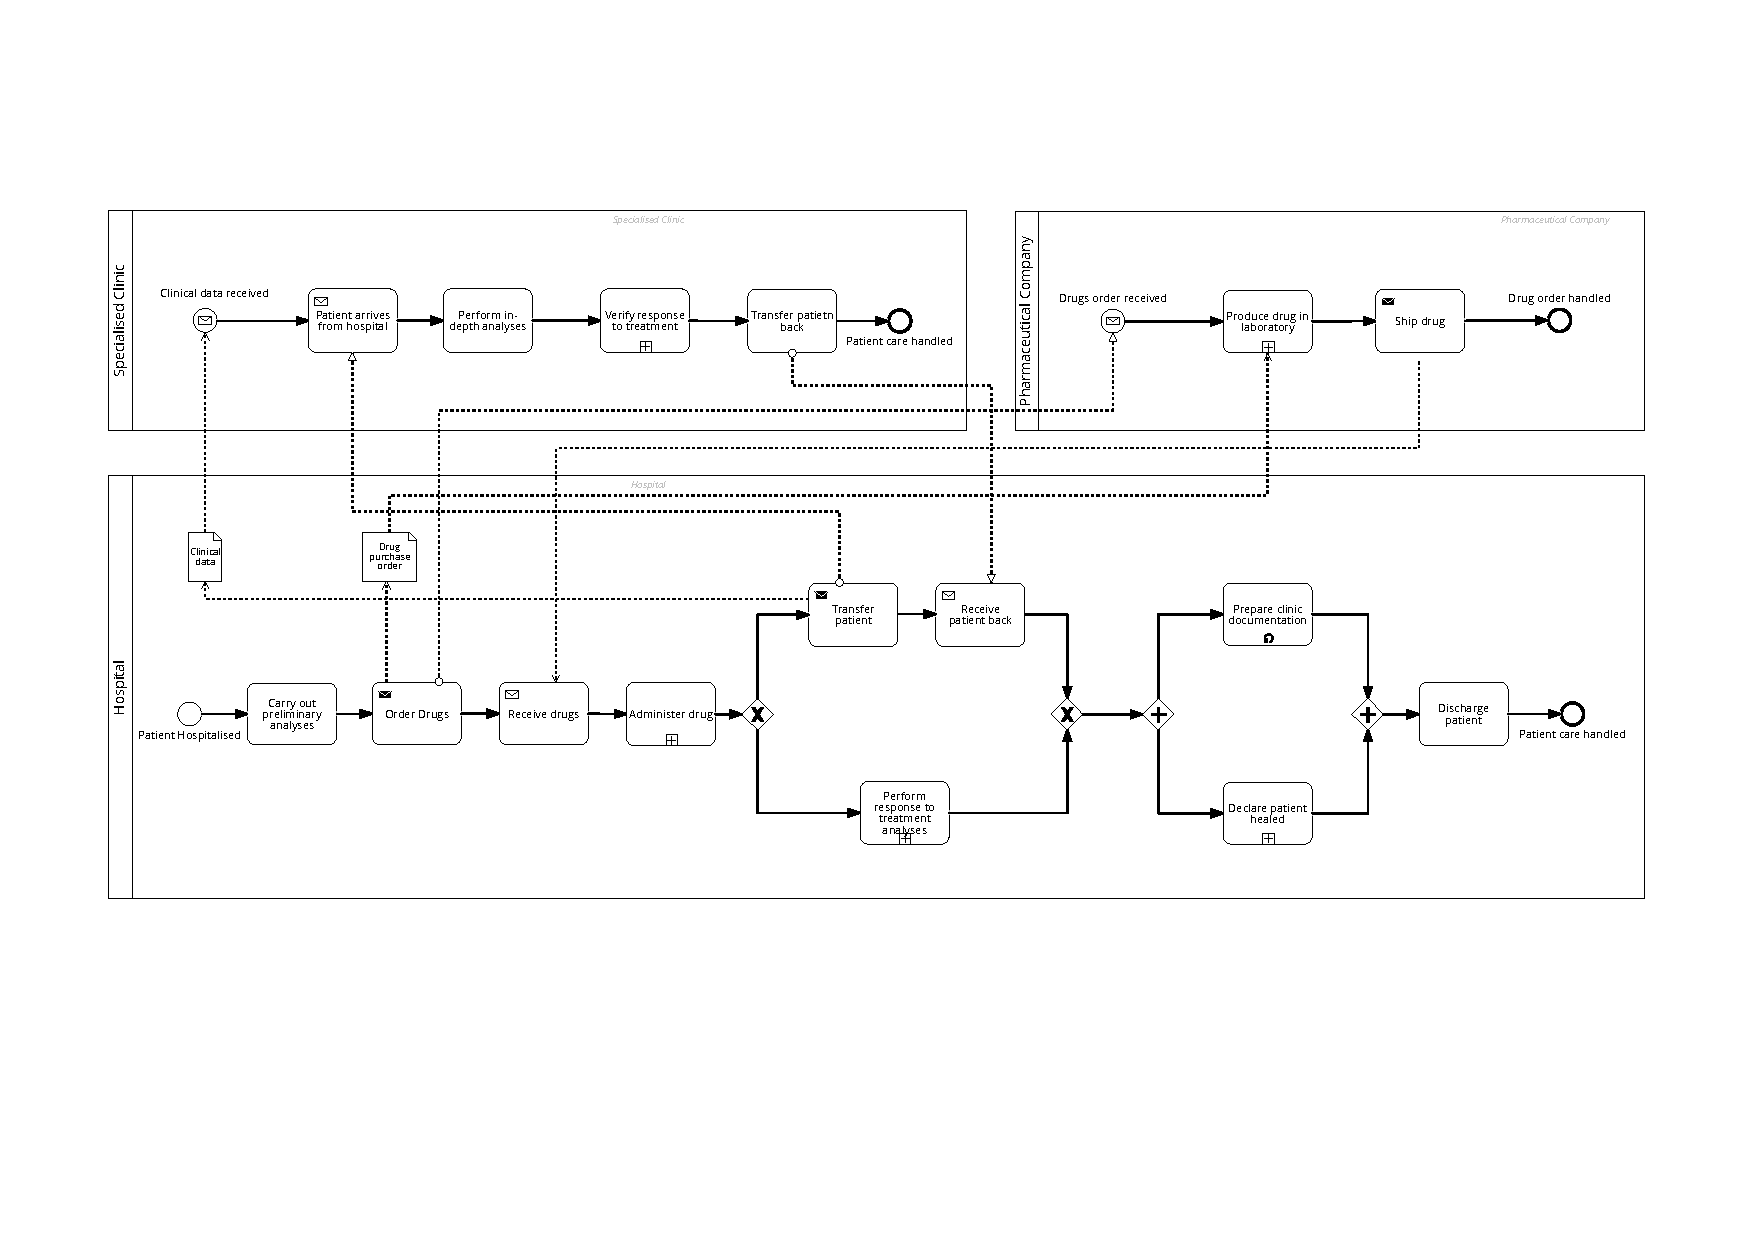
\includegraphics[width=0.9\linewidth]{content/figures/healthcarescenario.pdf}
\caption{BPMN Healthcare Scenario}
\label{fig:BPMN_Healthcare}
\end{figure}

\begin{table}[t]
\begin{tabular}{|lll|l|lll|l|lll|}
\cline{1-3} \cline{5-7} \cline{9-11}
\multicolumn{3}{|l|}{Hospital}                                               &  & \multicolumn{3}{l|}{Pharmaceutical company}                                 &  & \multicolumn{3}{l|}{Specialised Clinic}                                     \\ \cline{1-3} \cline{5-7} \cline{9-11} 
\multicolumn{1}{|l|}{Trace id} & \multicolumn{1}{l|}{Event name} & Timestamp &  & \multicolumn{1}{l|}{Trace id} & \multicolumn{1}{l|}{Event name} & Timestamp &  & \multicolumn{1}{l|}{Trace id} & \multicolumn{1}{l|}{Event name} & Timestamp \\ \cline{1-3} \cline{5-7} \cline{9-11} 
\multicolumn{1}{|l|}{}         & \multicolumn{1}{l|}{}           &           &  & \multicolumn{1}{l|}{}         & \multicolumn{1}{l|}{}           &           &  & \multicolumn{1}{l|}{}         & \multicolumn{1}{l|}{}           &           \\ \cline{1-3} \cline{5-7} \cline{9-11} 
\multicolumn{1}{|l|}{}         & \multicolumn{1}{l|}{}           &           &  & \multicolumn{1}{l|}{}         & \multicolumn{1}{l|}{}           &           &  & \multicolumn{1}{l|}{}         & \multicolumn{1}{l|}{}           &           \\ \cline{1-3} \cline{5-7} \cline{9-11} 
\end{tabular}
\end{table}

\begin{table}[t]
\begin{tabular}{lll}
\hline
\multicolumn{3}{|l|}{Hospital}                                                                             \\ \hline
\multicolumn{1}{|l|}{Trace id} & \multicolumn{2}{l|}{Trace}                                                \\ \hline
\multicolumn{1}{|l|}{0}        & \multicolumn{2}{l|}{\textless CPA, OD, RD, AD, PRM \textgreater{}}        \\ \hline
                               &                                      &                                    \\ \hline
\multicolumn{3}{|l|}{Pharmaceutical Company}                                                               \\ \hline
\multicolumn{1}{|l|}{Trace id} & \multicolumn{2}{l|}{Trace}                                                \\ \hline
\multicolumn{1}{|l|}{0}        & \multicolumn{2}{l|}{\textless BA, TI, MÒ, GI \textgreater{}}              \\ \hline
                               &                                      &                                    \\ \hline
\multicolumn{3}{|l|}{Specialised Clinic}                                                                   \\ \hline
\multicolumn{1}{|l|}{Trace id} & \multicolumn{2}{l|}{Trace}                                                \\ \hline
\multicolumn{1}{|l|}{0}        & \multicolumn{2}{l|}{\textless{}CT, QE, BTL, ASM, RTB, CDO \textgreater{}} \\ \hline
\end{tabular}
\end{table}

\section{Motivating Scenario}\label{sec:motivating}
Cooperation between different structures is crucial in the medical field, and many processes are frequently outsourced. In our running example, we consider a simplified healthcare scenario in which an hospitalization process involves the cooperation of three organizations, namely, the \texttt{Hospital}, the \texttt{Pharmaceutical Organization}, and the \texttt{Specialized Clinic}. We explain the process depicted in the BPMN diagram in \cref{fig:BPMN_Healthcare} as follows.
Preliminary examinations are carried out when a patient enters the \texttt{Hospital}. Then, the \texttt{Hospital} orders the drugs needed to treat the patient from the \texttt{Pharmaceutical Company}. The \texttt{Pharmaceutical Company} receives the order, produces the drugs in the laboratory, and sends them back to the \texttt{Hospital}. The \texttt{Hospital} manages the drugs received and verifies whether the patient can be treated internally. Patients requiring special care are transferred to the \texttt{Specialized Clinic} where more in-depth checks are carried out. Once the \texttt{Specialized Clinic} has verified the response to the alternative treatment, the patient is transferred to the \texttt{Hospital} to prepare the dehospitalization. Before discharging the patient, the \texttt{Hospital} prepares the necessary clinical documentation. In addition, the \texttt{Hospital} also carries out analysis checks. Finally, the \texttt{Hospital} discharges the patient.

The \texttt{Hospital}, the  organizations record the events belonging to different process instances in the traces of their event logs. In \cref{fig:BPMN_Healthcare}, we propose as an example two possible traces scattered across the three organizations. Traces of different organizations having the same ID are in the same process instance. TO BE CONTINUED ONCE WE HAVE THE IMAGE.\todo[]{Add two trace examples below the bpmn.}

%Any organization in the collaboration environment can request to perform process mining operations. For instance, the hospital cooperates with the specialized clinic and the pharmaceutical company, it can decide at any time to analyze the entire process by considering data from all three partners to provide an overview. The hospital requests the necessary data from all companies participating in the cooperation. All companies will send their process data in event log form. To mine all data together, the hospital must merge the event logs received. Once the event log has been merged, the hospital can proceed with the execution of the mining algorithm to analyze the entire process.

%TRACE 555

%Patient hospitalised, Carry out preliminary analyses , Order drugs, Receive drugs, Administer drug, Transfer the patient to chosen specialised clinic, Receive the patient back from specialised clinic, Declare patient healed, Prepare clinic documentation, Discharge patient

% ()Receive drugs order from hospital (2022-12-15T09:30:00Z), Produce new drugs in laboratory (2022-12-15T11:30:00Z),  Ship drugs to hospital (2022-12-15T13:30:00Z)

% Specialised: Patient arrives from hospital (2022-12-16T00:30:00Z), Perform more in-depth analyses (2022-12-16T02:30:00Z), Perform treatment (2022-12-16T04:30:00Z), Verify response to alternative treatment (2022-12-16T05:30:00Z), Transfer patient back to hospital (2022-12-16T06:30:00Z)
